\begin{figure}[htb]
\vspace{1mm}
\centering
%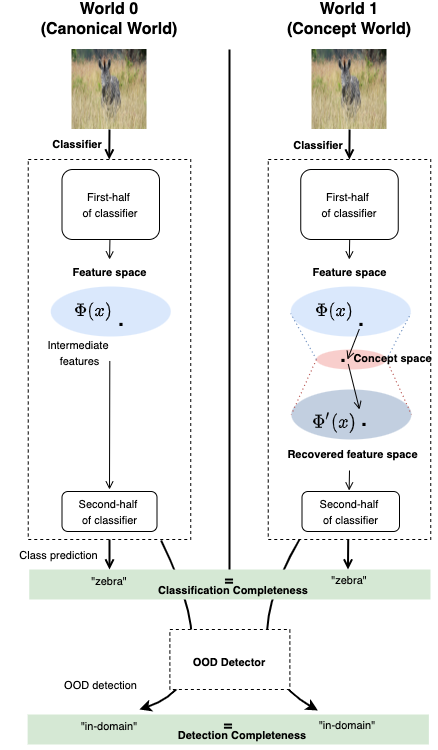
\includegraphics[width=0.45\textwidth]{figures/completeness.png}
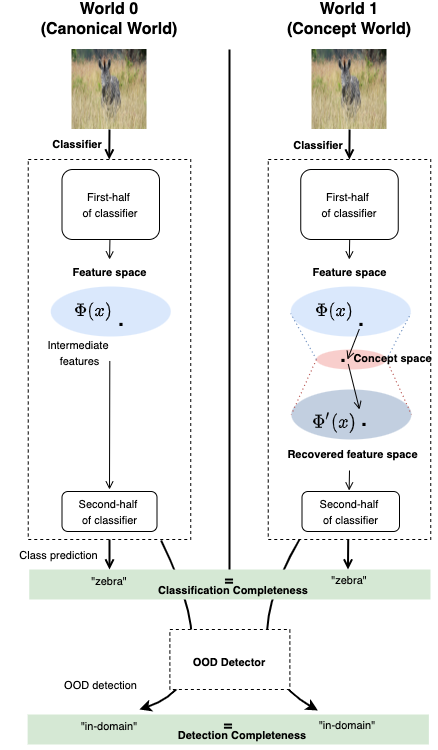
\includegraphics[scale=0.35]{figures/completeness.png}
%\vspace{-2mm}
\caption{\small \jihye{caption}}
\vspace{-5mm}
\label{fig:detection-completeness}
\end{figure}

\section{Proposed Method}
% \subsection{Evaluation metrics}
Given a trained DNN classifier $\bff$ and a trained OOD detector $\calD_\gamma$, our goal is to learn a set of concepts that can provide explanations for the predictions of the classifier and detector.
To this end, we first propose new metrics for quantifying a set of learned concepts, followed by a general framework for learning a set of concepts.

\subsection{Classifier and Detector in the Concept World}
\jihye{Classifier and Detector in Two Worlds}
\jihye{itemize and define world 0: , world 1}
For an input $\bfx$, consider the feature representation $\bfphi(\bfx)$, the output at a specific layer of the DNN classifier.
Without loss of generality, we focus on a convolutional layer with $\,\bfphi(\bfx) \in \reals^{a \times b \times d}$, where $d$ is the number of channels (\eg $d = 2048$), $a$ and $b$ are the filter size (\eg $a = b = 5$). Let $\bfc_i \in \reals^d, ~i = 1, \cdots, m$ denote the set of concept vectors (typically $m \ll d$).
The concept score corresponding to concept $i$ is the inner-product between the feature representation and the concept vector, \ie $\bfv_{\bfc_i}(\bfx) = \langle \bfphi(\bfx), \bfc_i \rangle \in \reals^{ab}$. This inner-product is defined as the concatenation over the $a \times b$ patch of the standard inner-products (between vectors) $\,\langle \bfphi^{p,q}(\bfx), \bfc_i \rangle \in \reals, ~\forall p, q \in [a] \times [b]$.
The vector of concept scores from all the concepts is defined simply as the concatenation of the individual concept scores, \ie $\VC(\bfx)^T = [\bfv_{\bfc_1}(\bfx)^T, \cdots, \bfv_{\bfc_m}(\bfx)^T] \in \reals^{abm}$.

We also define a dimension-reduced version of the concept score vector that takes the maximum of the inner-product over each $a \times b$ patch (instead of concatenating them) as follows: $\TVC(\bfx)^T = [\widetilde{v}_{\bfc_1}(\bfx), \cdots, \widetilde{v}_{\bfc_m}(\bfx)] \in \reals^m$, where $\widetilde{v}_{\bfc_i}(\bfx) = \max_{p, q} |\langle \bfphi^{p,q}(\bfx), \bfc_i \rangle|$. 
As mentioned earlier, this reduction operation is done to capture the most important correlations from each patch.

Given our assumption that the concept score vector is a sufficient statistic for the prediction of both the classifier and the detector, we define a mapping $\,\bfg : \reals^{abm} \mapsto \reals^{a \times b \times d}$ that reconstructs the feature representation at layer $\ell$ from the concept score vector.
To be precise, let $\,\recphi(\bfx) = \bfg(\VC(\bfx))$ define the reconstructed feature representation.
The mapping $\bfg$ is realized using a fully-connected neural network, whose parameters are optimized as part of the concept learning. This idea is explained in Fig.~\ref{fig:detection-completeness}.

\mypara{Classifier in the concept world.}
Given the original DNN classifier $\bff = \bfh \circ \bfphi$, we define the classifier in the ``concept world'' based on the reconstructed representation as
\begin{equation}
\label{equ:classifier_concept}
\fcon(\bfx) ~:=~ \bfh(\recphi(\bfx)) ~=~ \bfh(\bfg(\VC(\bfx))).
\end{equation}

\mypara{Detector in the concept world.}
Given an OOD detector $\calD_\gamma(\bfx, \bff)$ with score function $S(\bfx, \bff)$ for the classifier $\bff = \bfh \circ \bfphi$, we define the corresponding detector and the score function in the ``concept world'' based on the reconstructed representation as
\begin{align}
\label{equ:detector_concept}
\Dcon(\bfx, \bff) \,&:=\, \calD_\gamma(\bfx, \bfh \circ \recphi) \,=\, \calD_\gamma(\bfx, \bfh \circ \bfg \circ \VC) \nonumber \\
\Scon(\bfx, \bff) \,&:=\, S(\bfx, \bfh \circ \recphi) \,=\, S(\bfx, \bfh \circ \bfg \circ \VC).
\end{align}
Given a sufficient set of concepts $\bfC$, the classifier in the concept world should be able to closely approximate the prediction performance of the original classifier.
Likewise, the detector in the concept world should be able to closely approximate the detection performance of the original detector.
In order to concretely quantify this notion, we next define a 
% completeness score for both the classifier and the detector.
completeness score for the set of concepts with respect to the classification task and the OOD detection task.


\subsection{Completeness Score for Concepts}
\label{sec:completeness_score}
Briefly mention need for/intuition behind classification completeness by \cite{yeh2019completeness}\\.\\.\\.
%
\begin{definition}
\label{def:completeness_class}
Given a trained DNN classifier $\bff = \bfh \circ \bfphi\,$ and a set of concept vectors $\bfC$, the {\em classification completeness score} with respect to an ID distribution $\Pin(\bfx, y)$ is defined as \cite{yeh2019completeness}
\begin{align}
\label{equ: completeness-classification}
    &\eta^{}_\bff(\bfC) ~:= \\ 
    &\frac{\textrm{sup}_\bfg \,\expec_{(\bfx, y) \sim \Pin} \indicator[ y = \argmax_{y'} h_{y'}(\recphi(\bfx)) ] ~-~ a_r}{\expec_{(\bfx, y) \sim \Pin} \indicator[y = \argmax_{y'} h_{y'}(\bfphi(\bfx))] ~-~ a_r} \nonumber
\end{align}
where $\recphi(\bfx) = \bfg(\bfv_{\bfC}(\bfx))$ is the feature representation reconstructed from the concept scores, and $a_r$ is the accuracy of random prediction (\ie $a_r = 1/L$ for $L$ classes).
\end{definition}
In the numerator, the maximization is over the parameters of the fully-connected neural network $\bfg$ that reconstructs the feature representation from the vector of concept scores.
The denominator of $\eta^{}_\bff(\bfC)$ is the accuracy of the classifier $\bff$, while the numerator is the maximum accuracy that can be achieved using the feature representation reconstructed from the concept-score vector.
In practice, the expectation is estimated using a held-out test dataset $\Dinte$ from the ID distribution.

% \jihye{Limitation of the above completeness for our purpose. Need for / intuition behind detection completeness. fig (\ref{fig:detection-completeness})} \\.\\.\\.\\.\\.
% \jihye{Full elaboration on the two-world game -- fig \ref{fig:detection-completeness}}

\begin{definition}
\label{def:completeness_detec}
Given a trained DNN classifier $\bff = \bfh \circ \bfphi$, a trained OOD detector with score function $S(\bfx, \bff)$, and a set of concept vectors $\bfC$, the {\em detection completeness score} with respect to ID distribution $\Pin(\bfx, y)$ and OOD distribution $\Pout(\bfx)$ is defined as
\begin{align}
\label{equ: completeness-detection}
    \eta^{}_{\bff, S}(\bfC) 
    ~:=~ \frac{\textrm{sup}_\bfg \,\textrm{AUC}(\bfh \circ \recphi) ~-~ b_r}{\textrm{AUC}(\bfh \circ \bfphi) ~-~ b_r},
\end{align}
where $\recphi(\bfx) = \bfg(\bfv_{\bfC}(\bfx))$ is the feature representation reconstructed from the concept scores, $\textrm{AUC}(\bff)$ is the area under the ROC curve of an OOD detector for $\bff$, defined as
\begin{align}
\label{equ:auroc_ideal}
\textrm{AUC}(\bff) ~:= \!\!\expec_{(\bfx, y) \sim \Pin} \expec_{\,\bfx^\prime \sim \Pout} \indicator\big[ S(\bfx, \bff) \,>\, S(\bfx^\prime, \bff) \big],
\end{align}
and $b_r = 0.5$ is the AUROC of a random detector.
\end{definition}
As with the classification completeness, the maximization in the numerator is over the parameters of the fully-connected network $\bfg$ that reconstructs the feature representation from the vector of concept scores.
In practice, $\textrm{AUC}(\bff)$ is estimated using held-out test datasets from both the ID and OOD. Given an ID test dataset $\Dinte$ and an OOD test dataset $\Doutte$, the sample estimate of $\textrm{AUC}(\bff)$ is given by
\begin{align*}
    \widehat{\textrm{AUC}}(\bff) \,=\, \frac{1}{|\Dinte|\,|\Doutte|} \!\!\mysum_{(\bfx, y) \in \Dinte} \mysum_{~\bfx^\prime \in \Doutte} \!\!\!\indicator\big[ S(\bfx, \bff) > S(\bfx^\prime, \bff) \big]. 
\end{align*}

Both the classification completeness and detection completeness scores have a range $[0, 1]$, and a value close to $1$ indicates that the set of concepts $\bfC$ are close to complete in characterizing the behavior of the classifier and/or the OOD detector.

\subsection{Concept Separability Score}
\label{sec:separability_score}
\iffalse

% \somesh{Assumptions: enforcing separability of each individual separability --> anyway leads to better separability with combined concepts}
% \somesh{First describe the problem -what we want to do. There are these possible methods..... We chose this because of what. It should never appear like magic.}
% \somesh{Some curve -- accuracy vs separability something like that}

\jihye{need for/intuition behind separablility. Full elaboration on the idea behind separability in concept space -- fig \ref{fig:detection-separability}.} Other than the completeness scores of Eq. (\ref{equ: completeness-classification}) and Eq. (\ref{equ: completeness-detection}), we also want the concept scores between ID and OOD data to be easily distinguishable. This notion is captured by the \textit{separability} metric in Eq. (\ref{equ: distinguishability}). 

\fi
An important property that we would like to impose on the set of learned concepts for the OOD detection task is that the ID data and OOD data be well separated in the dimension-reduced concept-score space.
The motivation behind this requirement is two-fold.
The first is that we would like the concept scores to be highly distinguishable between the ID and OOD data (\eg Fig.~\ref{fig:detection-separability}), in order to effectively interpret the detector's decisions.
The second is that we would like the detector in the concept world Eq. (\ref{equ:detector_concept}) to have performance close to that of the original detector, which requires that the distribution of detector scores $\Scon(\cdot)$ from ID and OOD data be well separated.
% maybe we should say requirement of high detection completeness here?
This in-turn translates to a requirement of good separability (between ID and OOD) in the projected concept-score space.

Formally, we would like the set of concept-score vectors from the ID class $\,V_{\textrm{in}}(\bfC) := \{\TVC(\bfx) \in \reals^m ~:~ \bfx \sim \Pin\}$ and set of concept-score vectors from the OOD class $\,V_{\textrm{out}}(\bfC) := \{\TVC(\bfx) \in \reals^m ~:~ \bfx \sim \Pout\}$ to be well separated.
Let $\,J_{\textrm{sep}}(V_{\textrm{in}}(\bfC), V_{\textrm{out}}(\bfC)) \in \reals$ define a general {\it measure of separability} between the two data subsets, such that a larger value corresponds to higher separability.
We will discuss specific choices for $J_{\textrm{sep}}$ that make it possible to tractable optimize the concept separability as part of the learning objective.

Class separability metrics have been well studied in the pattern recognition literature, particularly for the two-class case~\cite{fukunaga1990separ}~\footnote{Note that the two classes correspond to ID and OOD data.}. 
Distributional divergences such as the Kullback-Leibler and Hellinger distance can be used when the probability distribution of the two classes are known, and the divergence is tractable to compute.
Non-parametric measures of class separability (\eg based on $k$-nearest neighbors) are also candidates here, but they are usually hard to optimize using gradient-based methods.
In order to obtain a closed-form expression for the class separability, it is common to make simplifying assumptions on the class-conditional density (\eg multivariate Gaussian per class).
% We next propose a binary class separability 

\mypara{Global Concept Separability.}
Motivated by Fisher's linear discriminant analysis (LDA), we explore the use of class-separability measures based on the within-class and between-class scatter matrices~\cite{murphy2012separ}.
The goal of LDA is to find a projection vector (direction) such that data from the two classes are maximally separated and form compact clusters when projected onto this vector. 
Rather than finding an optimal projection direction, we are more interested in ensuring that the concept-score vectors from the ID and OOD data have high separability.
Given the set of concept-score vectors from the ID data $V_{\textrm{in}}(\bfC)$ and OOD data $V_{\textrm{out}}(\bfC)$, consider their within-class and between-class scatter matrices defined as
\begin{align}
\label{eq:scatter_matrices}
\bfS_w ~&= \mysum_{\bfv \in V_{\textrm{in}}(\bfC)} (\bfv \,-\, \bfmu_{\textrm{in}})\,(\bfv \,-\, \bfmu_{\textrm{in}})^T \nonumber \\
&+ \mysum_{\bfv \in V_{\textrm{out}}(\bfC)} (\bfv \,-\, \bfmu_{\textrm{out}})\,(\bfv \,-\, \bfmu_{\textrm{out}})^T, \\
%
\bfS_b ~&=~ (\bfmu_{\textrm{out}} \,-\, \bfmu_{\textrm{in}})\,(\bfmu_{\textrm{out}} \,-\, \bfmu_{\textrm{in}})^T,
\end{align}
where $\bfmu_{\textrm{in}}$ and $\bfmu_{\textrm{out}}$ are the mean concept-score vectors corresponding to the ID and OOD data respectively.
We define the following separability metric between based on the generalized eigenvalue equation solved by Fisher's LDA~\cite{fukunaga1990separ, murphy2012separ}:
\begin{align}
\label{eq:separability_trace}
&J_{\textrm{sep}}(V_{\textrm{in}}(\bfC), V_{\textrm{out}}(\bfC)) ~=~ \textrm{tr}\big[\bfS_w^{-1} \,\bfS_b\big] \nonumber \\
% &=~ \textrm{tr}\big[\bfS_w^{-1} \,(\bfmu_{\textrm{out}} \,-\, \bfmu_{\textrm{in}})\,(\bfmu_{\textrm{out}} \,-\, \bfmu_{\textrm{in}})^T\big] \nonumber \\
&=~ (\bfmu_{\textrm{out}} \,-\, \bfmu_{\textrm{in}})^T \,\bfS_w^{-1} \,(\bfmu_{\textrm{out}} \,-\, \bfmu_{\textrm{in}}).
\end{align}
Maximizing the above metric is equivalent to maximizing the sum of eigenvalues of the matrix $\,\bfS_w^{-1} \,\bfS_b$, which in-turn ensures a large between-class separability and a small within-class separability for the ID and OOD concept scores.
We refer to this as a {\em global concept separability} metric because it does not analyze the separability between the ID and OOD data on a per-class level.
% it analyzes the ID and OOD data from all the $L$ classes.

\jihye{Check if the motivation for "multivariate" separability is conveyed here.}

\mypara{Connection to the Bhattacharya distance.}
We note that the separability metric in Eq. (\ref{eq:separability_trace}) is closely related to the Bhattacharya distance~\cite{bhattacharyya1943measure} for the special case when the concept scores from both ID and OOD data follow a multivariate Gaussian density. The Bhattacharya distance is a well known measure of divergence between two probability distributions, and it has the nice property of being an upper bound to the Bayes error rate in the two-class case~\cite{fukunaga1990bhatta}. For the special case when the concept scores from both ID and OOD data follow a multivariate Gaussian with a shared covariance matrix, it can be shown that the Bhattacharya distance reduces to the separability metric in Eq. (\ref{eq:separability_trace}) (ignoring scale factors). 

\iffalse

We sometimes denote $J_{\textrm{sep}}(V_{\textrm{in}}(\bfC), V_{\textrm{out}}(\bfC))$ as $J_{\textrm{sep}}(\bfC)$ for brevity.
Assumption of unimodal distribution; when this assumption may not be appropriate in some cases. 

\fi


\mypara{Per-Class Concept Separability.}
% Conditioned on a given predicted class
So far, we have focused on the separability between the concept scores of ID and OOD data without considering the class prediction of the classifier.
However, it may be more appropriate to impose high separability between the concept scores on a per-class level. In other words, we would like the concept scores of ID and OOD data predicted by the classifier into any given class $y \in [L]$ to be well separated.
Consider the set of concept-score vectors from ID data that are predicted into class $y$: $V^{y}_{\textrm{in}}(\bfC) := \{\TVC(\bfx) \in \reals^m ~:~ \bfx \sim \Pin, ~\widehat{y}(\bfx) = y\}$. 
Likewise, define for the OOD data $\,V^{y}_{\textrm{out}}(\bfC) := \{\TVC(\bfx) \in \reals^m ~:~ \bfx \sim \Pout, ~\widehat{y}(\bfx) = y\}$. 
We can extend the definition of the separability metric for a given predicted class $y \in [L]$ as follows
\begin{align}
\label{eq:separability_trace_per_class}
&J_{\textrm{sep}}(V^{y}_{\textrm{in}}(\bfC), V^{y}_{\textrm{out}}(\bfC)) ~=~ \textrm{tr}\big[(\bfS^{y}_w)^{-1} \,\bfS^y_b\big] \nonumber \\
&=~ (\bfmu^y_{\textrm{out}} \,-\, \bfmu^y_{\textrm{in}})^T \,(\bfS^y_w)^{-1} \,(\bfmu^y_{\textrm{out}} \,-\, \bfmu^y_{\textrm{in}}).
\end{align}
The scatter matrices $\bfS^y_w$ and $\bfS^y_b$ are defined similar to Eq. (\ref{eq:scatter_matrices}), using the per-class subset of concept scores $V^{y}_{\textrm{in}}(\bfC)$ or $V^{y}_{\textrm{out}}(\bfC)$, and the mean concept-score vectors from the ID and OOD data are also defined at a per-class level.

\jayaram{Need to say something more here. About how the global and per-class separability metrics are used.}

We sometimes use the notation $J_{\textrm{sep}}(\bfC)$ instead of $J_{\textrm{sep}}(V_{\textrm{in}}(\bfC), V_{\textrm{out}}(\bfC))$ and $J^y_{\textrm{sep}}(\bfC)$ instead of $J_{\textrm{sep}}(V^{y}_{\textrm{in}}(\bfC), V^{y}_{\textrm{out}}(\bfC))$ for brevity.

% In practice, a held-out validation dataset is used
% Define shorthand notations for the separability metrics.


\iffalse

% Separability literature (BC distance... assumptions.. special case: trace)
% \\.\\.\\.\\.\\.\\.\\.\\.

Given datasets $D_{\text{in}}^{l} = \{(\bfx_i, y_i) | y_i = l\}_{i=1}^{N_{in}^{l}}$ and $D_{\text{out}}^{l} = \{\bfx_i | y_i = l\}_{i=1}^{N_{out}^{l}}$, for each concept $k = 1, 2, ..., m$ and class label $l = 1, 2, ..., L$.
\begin{enumerate}
\item First, we compute means of concept scores for each concept: for ID cluster, $\mu_{in}^{l, k} = \frac{1}{N_{in}^l}\sum_{\bfx_i \in D^{l}_{in}} v_{\bfc_k}(\bfx_i)$ and for OOD cluster, $\mu_{out}^{l, k} = \frac{1}{N_{out}^l}\sum_{\bfx_i \in D^{l}_{out}} v_{\bfc_k}(\bfx_i)$ where $v_{\bfc_k}(\bfx_i)$ is the score with respect to the $k$-th concept $\bfc_k$.
We desire $\mu_{in}^{l, k}$ and $\mu_{out}^{l, k}$ to be as far as possible to each other.
\item Second, we compute intra-cluster scatters for each concept: for ID cluster, $s_{in}^{l, k} = \sum_{\bfx_i \in D^{l}_{in}} (v_{\bfc_k}(\bfx_i) - \mu_{in}^k)^2$ and for OOD cluster, $s_{out}^k = \sum_{\bfx_i \in D^{l}_{out}} (v_{\bfc_k}(\bfx_i) - \mu_{out}^k)^2$.
We desire $s_{in}^{l,k}$ and $s_{out}^{l,k}$ to be as small as possible.
\item Then the separability between the ID cluster and OOD cluster is measured as follows,
\begin{equation*}
    J^l(\bfc_k) = \frac{(\mu_{in}^k - \mu_{out}^k)^2}{(s_{in}^k + s_{out}^k)}
\end{equation*}
\begin{equation}
\label{equ: separability}
    J(\bfC) = \frac{1}{L \cdot m}\sum_{l=1}^L\sum_{k=1}^m J^l(\bfc_k)
\end{equation}
Higher score for $J(\bfC)$ indicates the better distinguishability between ID concept scores and OOD concept scores.
\end{enumerate}

Note the close relation to Fisher Linear Discriminant (FLD). FLD finds the optimal projection from high resolution input data into low dimensional representations that maximizes the separability between classes.
Let $\{\bfphi_1, \bfphi_2, .., \bfphi_n\}$ be $d$-dimensional samples that belong to one of binary classes, $y_i = \{0, 1\}$. \jihye{notation for detection vs notation for classification -- clarify!}
$\bfphi_i$ is the feature representation at layer $l$ flattened into $d$-dimensional vector: $\bfphi_i = \phi(\bfx_i)$.
Let $\bfv$ be a unit vector in the $d$-dimensional space and $z_i = \bfv\cdot\bfphi_i$ is the projection of $\bfphi_i$ into a one dimensional subspace.
Let $\mu_0 = \frac{1}{n_0}\sum_{z_i: y_i = 0}^{n_0} z_i = \bfv \cdot (\frac{1}{n_0}\sum_{\bfphi_i: y_i = 0}^{n_0} \bfphi_i)$ be the mean of projected values for class 0 and similarly, $\mu_1$ be the mean for class 1.
Define scatter for class 0 as $s_0 = \sum_{z_i: y_i = 0}^{n_0} (z_i - \mu_0)^2$ and similarly, $s_1$ is the scatter for class 1.
$s_0$ can be rewritten in a vector form as,
\begin{align*}
    s_0 &= \sum_{z_i: y_i = 0}^{n_0} (z_i - \mu_0)^2 = \sum_{\bfphi_i: y_i = 0}^{n_0} (\bfv \cdot (\bfphi_i - \bfmu_0))^2 \\
    &= \bfv^\mathsf{T} \cdot \left \Big[ \sum_{\bfphi_i: y_i = 0}^{n_0} (\bfphi_i - \bfmu_0) \cdot (\bfphi_i - \bfmu_0)^\mathsf{T} \right \Big] \cdot \bfv
\end{align*}
where $\bfmu_0 = \frac{1}{n_0}\sum_{\bfphi_i: y_i = 0}^{n_0} \bfphi_i$ is the sample mean for class 0.
Let $S_w$ be the within class scatter matrix: $S_w = \sum_{\bfphi_i: y_i = 0}^{n_0} (\bfphi_i - \bfmu_0) \cdot (\bfphi_i - \bfmu_0)^\mathsf{T} + \sum_{\bfphi_i: y_i = 1}^{n_1} (\bfphi_i - \bfmu_1) \cdot (\bfphi_i - \bfmu_1)^\mathsf{T}$. Then FLD measures the separability with respect to $\bfv$ as, 
\begin{equation}
    \label{equ: FLD}
    J_{Fisher}(\bfv) = \frac{(\mu_0 - \mu_1)^2}{(s_0 + s_1)} = \frac{\bfv^\mathsf{T} \cdot (\bfmu_0 - \bfmu_1)(\bfmu_0 - \bfmu_1)^\mathsf{T} \cdot \bfv }{\bfv^\mathsf{T} \cdot S_w \cdot \bfv}
\end{equation}
FLD finds $\widetilde{\bfv}$ such that $\frac{d J(\widetilde{\bfv})}{d \bfv} = 0$ for the optimal projection with maximum separability: $\widetilde{\bfv} = S_w^{-1}(\bfmu_0 - \bfmu_1)$.

Finally, our distinguishability index given a set of concept vectors $\bfC = \{\bfc_1, \bfc_2, ..., \bfc_m\}$ is defined as,
\begin{equation}
    \label{equ: distinguishability}
    S(\bfC) = \frac{J(\bfC)}{J_{Fisher}(\widetilde{\bfv})}
\end{equation}
% Guan et al. introduces Distance-based Separability Index (DSI) that measures how the distribution of intra-class distance (ICD) resembles the distribution of between-class distance (BCD) through statistical testing ~\cite{separability}. As the two classes are more separable, ICD and BCD are more distinguishable. 
% They verify the DSI to be more effective in measuring the separability of both synthetic and real-world datasets, compared to other separability indices such as Fisher discriminant ratio, neighborhood measures and linearity measures.
% We adopt DSI to quantify how distinguishable the ID concept scores and OOD concept scores are.
% Given $D_{\text{in}}^{test} = \{(\bfx_i, y_i)\}_{i=1}^{N_{in}}$ and $D_{\text{out}}^{test} = \{\bfx_i\}_{i=1}^{N_{out}}$, and a set of concept vectors $\bfC = \{\bfc\}_i^m$, we compute separability score between ID and OOD:
% \begin{enumerate}
%     \item First, we prepare $S_{in} = \{s_1, s_2, ..., s_{N_{in}}~|~s_i = v_\bfC(\bfx_i), \bfx_i \in D^{test}_{in}\}$ and $S_{out} = \{s_1, s_2, ..., s_{N_{out}}~|~s_i = v_\bfC(\bfx_i), \bfx_i \in D^{test}_{out}\}$. These are the set of concept scores for ID and OOD data, respectively.
    
%     \item ICD set for ID data, $\{d_{in}\}$ is a set of $l_2$ distances between any two points in $S(D_{\text{in}}^{test})$: $\{d_{in}\} = \{||s_i - s_j||_2 ~|~ s_i, s_j \in S_{in}; s_i \neq s_j\}$.
%     Likewise, $\{d_{out}\}$ is the ICD set for OOD data.
    
%     \item BCD set between ID and OOD data, $\{d_{in, out}\}$ is the set of $l_2$ distances between any two points from different distribution (ID and OOD): $\{d_{in, out}\} = \{||s_{in} - s_{out}||_2 ~|~ s_{in} \in S_{in}, s_out \in S_{out}\}$.
    
%     \item Then, the similarity between the ICD and BCD sets are computed using the Kolmogorov-Smirnov (KS) distance:
%     \[k_{in} = KS(\{d_{in}\}, \{d_{in, out}\}), \textrm{and}~ k_{out} = KS(\{d_{out}\}, \{d_{in, out}\})\]
%     \item Finally, the DSI of ID and OOD data is computed by averaging the two KS distances as follows,
%     \begin{equation}
%         \label{equ: separability}
%         DSI(D_{\text{in}}^{test}, D_{\text{out}}^{test}) = \frac{(k_{in} + k_{out})}{2}
%     \end{equation}
% \end{enumerate}

\fi


\subsection{Proposed Concept Learning Algorithm}
\label{sec:concept_learning}

\label{alg:concept_learning}
\begin{algorithm}
\caption{Learning concepts for OOD detector}
\begin{algorithmic}[1]
  \INPUT: Entire training set $\Dtr = \{\Dintr, \Douttr\}$, entire validation set $\Dval = \{\Dinval, \Doutval\}$, classifier $\bff$, detector $\calD$;
  \OUTPUT: $\bfC$, $g$
  \STATE initialize $\bfC$ and parameters of $g$;
  \STATE identify threshold $\gamma$ for $\calD_\gamma(\bfx, \bff)$ on $\Dval$, and prepare $\widehat{\Dinval}$ and $\widehat{\Doutval}$;
  \FOR{$i = 0, 1, 2, ... $}
    \STATE 
    \STATE 
	\STATE 
    \STATE Update $g$ and $\bfC$ using Eqn. \ref{equ: concept learning}: \\
	\quad Option I: 
  \ENDFOR
%   \RETURN $g$
\end{algorithmic}
\end{algorithm}

In this section, we develop our proposed concept learning objective that aims to find a set of concepts $\bfC = \{\bfc_1, \bfc_2, ..., \bfc_m\}$ and a mapping $\bfg$ (parameterized by a neural network) that have the following properties: 1) high detection completeness w.r.t the given OOD detector; 2) high classification completeness w.r.t the DNN classifier; and 3) high separability in the concept-score space between the samples detected as ID and the samples detected as OOD by the detector. 

\mypara{Limitation of Previous Work.} 
\cite{yeh2019completeness} 
The baseline concept learning objective by \cite{yeh2019completeness} aims to find a set of concepts $\bfC$ and a mapping $\bfg$ (parameterized by a neural network) that jointly maximize the recovered accuracy of the classifier in the concept world.
% to maximize the completeness of the learned concepts $\bfC = \{\bfc_1, \bfc_2, ..., \bfc_m\}$ for the classification task as follows,
\begin{equation}
\label{equ: baseline}
    \argmax_{\bfC, \bfg} \expec_{(\bfx, y) \sim \Pin}\!\!\big[ \log h_y(\bfg(\VC(\bfx))) \big] ~+~ \lambda_{\textrm{expl}}\, R_{\textrm{expl}}(\bfC),
\end{equation}
where $R_{\textrm{expl}}(\bfC)$ is a regularization term used to ensure that the learned concept vectors have high spatial coherancy and low redundancy (among themselves). It is defined as
\begin{align}
\label{equ:regularizer_expl}
    R_{\textrm{expl}}(\bfC) ~&=~ \frac{1}{m\,K} \mysum_{k=1}^m \mysum_{\bfx^\prime \in T_{\bfc_k}} \langle \bfphi(\bfx^\prime), \bfc_k \rangle \nonumber \\
    &-~ \frac{1}{m \,(m - 1)} \mysum_{j=1}^m \mysum_{k=j + 1}^m \langle \bfc_j, \bfc_k \rangle.
\end{align}
Here $T_{\bfc_k}$ is the set of $K$-nearest neighbor patches of the concept vector $\bfc_k$ from the ID training set $\Dintr$.
 


Unfortunately, the objective in Eq. (\ref{equ: baseline}) does not guarantee that the recovered feature representation $\recphi(\bfx)$ would match the original feature representation $\bfphi(\bfx)$.
Even when the recovered accuracy matches the original classification accuracy, if $\recphi(\bfx)$ and $\bfphi(\bfx)$ are not sufficiently close, the representations at the penultimate layer would vary a lot, leading to unmatched detection results by $\mathcal{D}$.
Hence, we include an additional regularization term that minimizes the $\ell_2$ distance 
% \begin{equation}
% \label{equ: baseline+l2}
%     \argmax_{\bfC, g} \, \text{log} \proba_{(\bfx, y) \sim D^{train}_{in}}[\, h_{y}(\hat{\phi}_{g, \bfC}(\bfx))] + \lambda_1 \cdot R_{coherency}(\bfC) + \lambda_2 \cdot
%     \expec_{\bfx \sim D_{train}^{in}}||\phi(\bfx) - \hat{\phi}_{g, \bfC}(\bfx))||_2
% \end{equation}
% \begin{equation}
% \label{equ: baseline+score}
%     \argmax_{\bfC, g} \, \log \proba_{(\bfx, y) \sim D^{train}_{in}}[\, h_{y}(\hat{\phi}_{g, \bfC}(\bfx))] ~+~ \lambda\, R_{coherency}(\bfC) ~-~ \alpha \expec_{\bfx \sim D_{train}^{in}} (\mathcal{D}(h(\hat{\phi}_{g, \bfC}(\bfx))) - \mathcal{D}(f(\bfx)))^2
% \end{equation}

% Let $D^{train} = \{D_{\text{in}}^{train} \cup D_{\text{out}}^{train}\}$, and data is drawn as $(\bfx, s) \sim D^{train}$ where $s \in \{0, 1\}$ is the groundtruth label of OOD detection.
%
% \begin{equation}
% \label{equ: baseline+separability}
%     \argmax_{\bfC, g} \, \log \proba_{(\bfx, y) \sim D^{train}_{in}}[\, h_{y}(\hat{\phi}_{g, \bfC}(\bfx))] ~+~ \lambda\, R_{coherency}(\bfC) ~+~ \beta \expec_{\bfx \sim D^{train}} J(\bfC)
% \end{equation}
%

\begin{align}
\label{equ: concept learning}
\argmax_{\bfC, g}\, &\log \proba_{(\bfx, y) \sim D^{train}_{in}}[\, h_{y}(\hat{\phi}_{g, \bfC}(\bfx))] ~+~ \lambda_{\textrm{expl}}\, R_{\textrm{expl}}(\bfC) \nonumber \\
&-~ \lambda_{\textrm{mse}}\, \expec_{\bfx \sim \Dtr} (\Dcon(\bfx, \bff) - \calD_\gamma(\bfx, \bff))^2 \nonumber \\
&-~ \lambda_{\textrm{norm}}\, \expec_{\bfx \sim \Dintr}||\bfphi(\bfx) - \recphi(\bfx)||^2 \nonumber \\
&+~ \lambda_{\textrm{sep}}~J(\bfC)
\end{align}
\jihye{shall we need some algorithm block?}
%
% Note that using \begin{align} ... \end{align} is a better way that using \begin{array}
% \begin{equation}
% \label{equ: concept learning}
% \begin{array}{l}
%     \argmax_{\bfC, g} \, \log \proba_{(\bfx, y) \sim D^{train}_{in}}[\, h_{y}(\hat{\phi}_{g, \bfC}(\bfx))] ~+~ \lambda\, R_{coherency}(\bfC) \hspace{20mm} \\
%     -~ \alpha\, \expec_{\bfx \sim D^{train}}\mathcal{D}(h(\hat{\phi}_{g, \bfC}(\bfx))) - \mathcal{D}(f(\bfx)))^2 
%     ~+~ \beta\, \expec_{\bfx \sim D^{train}} J(\bfC) \\
%     -~ \gamma\, \expec_{\bfx \sim D^{train}}||\phi(\bfx) - \hat{\phi}_{g, \bfC}(\bfx))||_2
% \end{array}
% \end{equation}

